% Options for packages loaded elsewhere
\PassOptionsToPackage{unicode}{hyperref}
\PassOptionsToPackage{hyphens}{url}
\PassOptionsToPackage{dvipsnames,svgnames,x11names}{xcolor}
%
\documentclass[
  letterpaper,
  DIV=11,
  numbers=noendperiod]{scrartcl}

\usepackage{amsmath,amssymb}
\usepackage{iftex}
\ifPDFTeX
  \usepackage[T1]{fontenc}
  \usepackage[utf8]{inputenc}
  \usepackage{textcomp} % provide euro and other symbols
\else % if luatex or xetex
  \usepackage{unicode-math}
  \defaultfontfeatures{Scale=MatchLowercase}
  \defaultfontfeatures[\rmfamily]{Ligatures=TeX,Scale=1}
\fi
\usepackage{lmodern}
\ifPDFTeX\else  
    % xetex/luatex font selection
\fi
% Use upquote if available, for straight quotes in verbatim environments
\IfFileExists{upquote.sty}{\usepackage{upquote}}{}
\IfFileExists{microtype.sty}{% use microtype if available
  \usepackage[]{microtype}
  \UseMicrotypeSet[protrusion]{basicmath} % disable protrusion for tt fonts
}{}
\makeatletter
\@ifundefined{KOMAClassName}{% if non-KOMA class
  \IfFileExists{parskip.sty}{%
    \usepackage{parskip}
  }{% else
    \setlength{\parindent}{0pt}
    \setlength{\parskip}{6pt plus 2pt minus 1pt}}
}{% if KOMA class
  \KOMAoptions{parskip=half}}
\makeatother
\usepackage{xcolor}
\setlength{\emergencystretch}{3em} % prevent overfull lines
\setcounter{secnumdepth}{-\maxdimen} % remove section numbering
% Make \paragraph and \subparagraph free-standing
\makeatletter
\ifx\paragraph\undefined\else
  \let\oldparagraph\paragraph
  \renewcommand{\paragraph}{
    \@ifstar
      \xxxParagraphStar
      \xxxParagraphNoStar
  }
  \newcommand{\xxxParagraphStar}[1]{\oldparagraph*{#1}\mbox{}}
  \newcommand{\xxxParagraphNoStar}[1]{\oldparagraph{#1}\mbox{}}
\fi
\ifx\subparagraph\undefined\else
  \let\oldsubparagraph\subparagraph
  \renewcommand{\subparagraph}{
    \@ifstar
      \xxxSubParagraphStar
      \xxxSubParagraphNoStar
  }
  \newcommand{\xxxSubParagraphStar}[1]{\oldsubparagraph*{#1}\mbox{}}
  \newcommand{\xxxSubParagraphNoStar}[1]{\oldsubparagraph{#1}\mbox{}}
\fi
\makeatother

\usepackage{color}
\usepackage{fancyvrb}
\newcommand{\VerbBar}{|}
\newcommand{\VERB}{\Verb[commandchars=\\\{\}]}
\DefineVerbatimEnvironment{Highlighting}{Verbatim}{commandchars=\\\{\}}
% Add ',fontsize=\small' for more characters per line
\usepackage{framed}
\definecolor{shadecolor}{RGB}{241,243,245}
\newenvironment{Shaded}{\begin{snugshade}}{\end{snugshade}}
\newcommand{\AlertTok}[1]{\textcolor[rgb]{0.68,0.00,0.00}{#1}}
\newcommand{\AnnotationTok}[1]{\textcolor[rgb]{0.37,0.37,0.37}{#1}}
\newcommand{\AttributeTok}[1]{\textcolor[rgb]{0.40,0.45,0.13}{#1}}
\newcommand{\BaseNTok}[1]{\textcolor[rgb]{0.68,0.00,0.00}{#1}}
\newcommand{\BuiltInTok}[1]{\textcolor[rgb]{0.00,0.23,0.31}{#1}}
\newcommand{\CharTok}[1]{\textcolor[rgb]{0.13,0.47,0.30}{#1}}
\newcommand{\CommentTok}[1]{\textcolor[rgb]{0.37,0.37,0.37}{#1}}
\newcommand{\CommentVarTok}[1]{\textcolor[rgb]{0.37,0.37,0.37}{\textit{#1}}}
\newcommand{\ConstantTok}[1]{\textcolor[rgb]{0.56,0.35,0.01}{#1}}
\newcommand{\ControlFlowTok}[1]{\textcolor[rgb]{0.00,0.23,0.31}{\textbf{#1}}}
\newcommand{\DataTypeTok}[1]{\textcolor[rgb]{0.68,0.00,0.00}{#1}}
\newcommand{\DecValTok}[1]{\textcolor[rgb]{0.68,0.00,0.00}{#1}}
\newcommand{\DocumentationTok}[1]{\textcolor[rgb]{0.37,0.37,0.37}{\textit{#1}}}
\newcommand{\ErrorTok}[1]{\textcolor[rgb]{0.68,0.00,0.00}{#1}}
\newcommand{\ExtensionTok}[1]{\textcolor[rgb]{0.00,0.23,0.31}{#1}}
\newcommand{\FloatTok}[1]{\textcolor[rgb]{0.68,0.00,0.00}{#1}}
\newcommand{\FunctionTok}[1]{\textcolor[rgb]{0.28,0.35,0.67}{#1}}
\newcommand{\ImportTok}[1]{\textcolor[rgb]{0.00,0.46,0.62}{#1}}
\newcommand{\InformationTok}[1]{\textcolor[rgb]{0.37,0.37,0.37}{#1}}
\newcommand{\KeywordTok}[1]{\textcolor[rgb]{0.00,0.23,0.31}{\textbf{#1}}}
\newcommand{\NormalTok}[1]{\textcolor[rgb]{0.00,0.23,0.31}{#1}}
\newcommand{\OperatorTok}[1]{\textcolor[rgb]{0.37,0.37,0.37}{#1}}
\newcommand{\OtherTok}[1]{\textcolor[rgb]{0.00,0.23,0.31}{#1}}
\newcommand{\PreprocessorTok}[1]{\textcolor[rgb]{0.68,0.00,0.00}{#1}}
\newcommand{\RegionMarkerTok}[1]{\textcolor[rgb]{0.00,0.23,0.31}{#1}}
\newcommand{\SpecialCharTok}[1]{\textcolor[rgb]{0.37,0.37,0.37}{#1}}
\newcommand{\SpecialStringTok}[1]{\textcolor[rgb]{0.13,0.47,0.30}{#1}}
\newcommand{\StringTok}[1]{\textcolor[rgb]{0.13,0.47,0.30}{#1}}
\newcommand{\VariableTok}[1]{\textcolor[rgb]{0.07,0.07,0.07}{#1}}
\newcommand{\VerbatimStringTok}[1]{\textcolor[rgb]{0.13,0.47,0.30}{#1}}
\newcommand{\WarningTok}[1]{\textcolor[rgb]{0.37,0.37,0.37}{\textit{#1}}}

\providecommand{\tightlist}{%
  \setlength{\itemsep}{0pt}\setlength{\parskip}{0pt}}\usepackage{longtable,booktabs,array}
\usepackage{calc} % for calculating minipage widths
% Correct order of tables after \paragraph or \subparagraph
\usepackage{etoolbox}
\makeatletter
\patchcmd\longtable{\par}{\if@noskipsec\mbox{}\fi\par}{}{}
\makeatother
% Allow footnotes in longtable head/foot
\IfFileExists{footnotehyper.sty}{\usepackage{footnotehyper}}{\usepackage{footnote}}
\makesavenoteenv{longtable}
\usepackage{graphicx}
\makeatletter
\def\maxwidth{\ifdim\Gin@nat@width>\linewidth\linewidth\else\Gin@nat@width\fi}
\def\maxheight{\ifdim\Gin@nat@height>\textheight\textheight\else\Gin@nat@height\fi}
\makeatother
% Scale images if necessary, so that they will not overflow the page
% margins by default, and it is still possible to overwrite the defaults
% using explicit options in \includegraphics[width, height, ...]{}
\setkeys{Gin}{width=\maxwidth,height=\maxheight,keepaspectratio}
% Set default figure placement to htbp
\makeatletter
\def\fps@figure{htbp}
\makeatother

\KOMAoption{captions}{tableheading}
\makeatletter
\@ifpackageloaded{caption}{}{\usepackage{caption}}
\AtBeginDocument{%
\ifdefined\contentsname
  \renewcommand*\contentsname{Table of contents}
\else
  \newcommand\contentsname{Table of contents}
\fi
\ifdefined\listfigurename
  \renewcommand*\listfigurename{List of Figures}
\else
  \newcommand\listfigurename{List of Figures}
\fi
\ifdefined\listtablename
  \renewcommand*\listtablename{List of Tables}
\else
  \newcommand\listtablename{List of Tables}
\fi
\ifdefined\figurename
  \renewcommand*\figurename{Figure}
\else
  \newcommand\figurename{Figure}
\fi
\ifdefined\tablename
  \renewcommand*\tablename{Table}
\else
  \newcommand\tablename{Table}
\fi
}
\@ifpackageloaded{float}{}{\usepackage{float}}
\floatstyle{ruled}
\@ifundefined{c@chapter}{\newfloat{codelisting}{h}{lop}}{\newfloat{codelisting}{h}{lop}[chapter]}
\floatname{codelisting}{Listing}
\newcommand*\listoflistings{\listof{codelisting}{List of Listings}}
\makeatother
\makeatletter
\makeatother
\makeatletter
\@ifpackageloaded{caption}{}{\usepackage{caption}}
\@ifpackageloaded{subcaption}{}{\usepackage{subcaption}}
\makeatother

\ifLuaTeX
  \usepackage{selnolig}  % disable illegal ligatures
\fi
\usepackage{bookmark}

\IfFileExists{xurl.sty}{\usepackage{xurl}}{} % add URL line breaks if available
\urlstyle{same} % disable monospaced font for URLs
\hypersetup{
  pdftitle={Lab 5},
  pdfauthor={Jazmin Hernandez},
  colorlinks=true,
  linkcolor={blue},
  filecolor={Maroon},
  citecolor={Blue},
  urlcolor={Blue},
  pdfcreator={LaTeX via pandoc}}


\title{Lab 5}
\author{Jazmin Hernandez}
\date{}

\begin{document}
\maketitle


\subsection{Reading in Data}\label{reading-in-data}

\begin{Shaded}
\begin{Highlighting}[]
\FunctionTok{library}\NormalTok{(data.table)}
\FunctionTok{library}\NormalTok{(dtplyr)}
\FunctionTok{library}\NormalTok{(dplyr)}
\end{Highlighting}
\end{Shaded}

\begin{verbatim}

Attaching package: 'dplyr'
\end{verbatim}

\begin{verbatim}
The following objects are masked from 'package:data.table':

    between, first, last
\end{verbatim}

\begin{verbatim}
The following objects are masked from 'package:stats':

    filter, lag
\end{verbatim}

\begin{verbatim}
The following objects are masked from 'package:base':

    intersect, setdiff, setequal, union
\end{verbatim}

\begin{Shaded}
\begin{Highlighting}[]
\FunctionTok{library}\NormalTok{(ggplot2)}
\NormalTok{met }\OtherTok{\textless{}{-}} \FunctionTok{read.csv}\NormalTok{(}\FunctionTok{file.path}\NormalTok{(}\StringTok{"\textasciitilde{}"}\NormalTok{, }\StringTok{"Github"}\NormalTok{, }\StringTok{"met\_all.gz"}\NormalTok{))}
\FunctionTok{head}\NormalTok{(met)}
\end{Highlighting}
\end{Shaded}

\begin{verbatim}
  USAFID  WBAN year month day hour min  lat      lon elev wind.dir wind.dir.qc
1 690150 93121 2019     8   1    0  56 34.3 -116.166  696      220           5
2 690150 93121 2019     8   1    1  56 34.3 -116.166  696      230           5
3 690150 93121 2019     8   1    2  56 34.3 -116.166  696      230           5
4 690150 93121 2019     8   1    3  56 34.3 -116.166  696      210           5
5 690150 93121 2019     8   1    4  56 34.3 -116.166  696      120           5
6 690150 93121 2019     8   1    5  56 34.3 -116.166  696       NA           9
  wind.type.code wind.sp wind.sp.qc ceiling.ht ceiling.ht.qc ceiling.ht.method
1              N     5.7          5      22000             5                 9
2              N     8.2          5      22000             5                 9
3              N     6.7          5      22000             5                 9
4              N     5.1          5      22000             5                 9
5              N     2.1          5      22000             5                 9
6              C     0.0          5      22000             5                 9
  sky.cond vis.dist vis.dist.qc vis.var vis.var.qc temp temp.qc dew.point
1        N    16093           5       N          5 37.2       5      10.6
2        N    16093           5       N          5 35.6       5      10.6
3        N    16093           5       N          5 34.4       5       7.2
4        N    16093           5       N          5 33.3       5       5.0
5        N    16093           5       N          5 32.8       5       5.0
6        N    16093           5       N          5 31.1       5       5.6
  dew.point.qc atm.press atm.press.qc       rh
1            5    1009.9            5 19.88127
2            5    1010.3            5 21.76098
3            5    1010.6            5 18.48212
4            5    1011.6            5 16.88862
5            5    1012.7            5 17.38410
6            5    1012.7            5 20.01540
\end{verbatim}

\begin{Shaded}
\begin{Highlighting}[]
\NormalTok{stations }\OtherTok{\textless{}{-}} \FunctionTok{fread}\NormalTok{(}\StringTok{"https://noaa{-}isd{-}pds.s3.amazonaws.com/isd{-}history.csv"}\NormalTok{)}
\NormalTok{stations }\OtherTok{\textless{}{-}} \FunctionTok{as.data.frame}\NormalTok{(stations)}
\NormalTok{stations}\SpecialCharTok{$}\NormalTok{USAF }\OtherTok{\textless{}{-}} \FunctionTok{as.integer}\NormalTok{(stations}\SpecialCharTok{$}\NormalTok{USAF)}
\end{Highlighting}
\end{Shaded}

\begin{verbatim}
Warning: NAs introduced by coercion
\end{verbatim}

\begin{Shaded}
\begin{Highlighting}[]
\NormalTok{stations}\SpecialCharTok{$}\NormalTok{USAF[stations}\SpecialCharTok{$}\NormalTok{USAF }\SpecialCharTok{==} \DecValTok{999999}\NormalTok{] }\OtherTok{\textless{}{-}} \ConstantTok{NA}
\NormalTok{stations}\SpecialCharTok{$}\NormalTok{CTRY[stations}\SpecialCharTok{$}\NormalTok{CTRY }\SpecialCharTok{==} \StringTok{""}\NormalTok{] }\OtherTok{\textless{}{-}} \ConstantTok{NA}
\NormalTok{stations}\SpecialCharTok{$}\NormalTok{STATE[stations}\SpecialCharTok{$}\NormalTok{STATE }\SpecialCharTok{==} \StringTok{""}\NormalTok{] }\OtherTok{\textless{}{-}} \ConstantTok{NA}
\end{Highlighting}
\end{Shaded}

\begin{Shaded}
\begin{Highlighting}[]
\NormalTok{stations }\OtherTok{\textless{}{-}} \FunctionTok{unique}\NormalTok{(stations[, }\FunctionTok{c}\NormalTok{(}\StringTok{\textquotesingle{}USAF\textquotesingle{}}\NormalTok{, }\StringTok{\textquotesingle{}CTRY\textquotesingle{}}\NormalTok{, }\StringTok{\textquotesingle{}STATE\textquotesingle{}}\NormalTok{)])}
\NormalTok{stations }\OtherTok{\textless{}{-}}\NormalTok{ stations[}\SpecialCharTok{!}\FunctionTok{is.na}\NormalTok{(stations}\SpecialCharTok{$}\NormalTok{USAF), ]}
\FunctionTok{head}\NormalTok{(stations, }\AttributeTok{n =} \DecValTok{4}\NormalTok{)}
\end{Highlighting}
\end{Shaded}

\begin{verbatim}
  USAF CTRY STATE
1 7018 <NA>  <NA>
2 7026   AF  <NA>
3 7070   AF  <NA>
4 8260 <NA>  <NA>
\end{verbatim}

\begin{Shaded}
\begin{Highlighting}[]
\CommentTok{\# Merging data}
\FunctionTok{merge}\NormalTok{(}
  \CommentTok{\# Data}
  \AttributeTok{x     =}\NormalTok{ met,      }
  \AttributeTok{y     =}\NormalTok{ stations, }
  \CommentTok{\# List of variables to match}
  \AttributeTok{by.x  =} \StringTok{"USAFID"}\NormalTok{,}
  \AttributeTok{by.y  =} \StringTok{"USAF"}\NormalTok{, }
  \CommentTok{\# Which obs to keep?}
  \AttributeTok{all.x =} \ConstantTok{TRUE}\NormalTok{,      }
  \AttributeTok{all.y =} \ConstantTok{FALSE}
\NormalTok{  ) }\SpecialCharTok{|\textgreater{}} \FunctionTok{nrow}\NormalTok{()}
\end{Highlighting}
\end{Shaded}

\begin{verbatim}
[1] 2385443
\end{verbatim}

\begin{Shaded}
\begin{Highlighting}[]
\NormalTok{stations }\OtherTok{\textless{}{-}}\NormalTok{ stations[}\SpecialCharTok{!}\FunctionTok{duplicated}\NormalTok{(stations}\SpecialCharTok{$}\NormalTok{USAF), ]}
\end{Highlighting}
\end{Shaded}

\begin{Shaded}
\begin{Highlighting}[]
\CommentTok{\# Fixed data dropping duplicate IDs from stations}
\NormalTok{met }\OtherTok{\textless{}{-}} \FunctionTok{merge}\NormalTok{(}
  \AttributeTok{x     =}\NormalTok{ met,      }
  \AttributeTok{y     =}\NormalTok{ stations, }
  \AttributeTok{by.x  =} \StringTok{"USAFID"}\NormalTok{,}
  \AttributeTok{by.y  =} \StringTok{"USAF"}\NormalTok{, }
  \AttributeTok{all.x =} \ConstantTok{TRUE}\NormalTok{,      }
  \AttributeTok{all.y =} \ConstantTok{FALSE}
\NormalTok{  )}
\FunctionTok{head}\NormalTok{(met[, }\FunctionTok{c}\NormalTok{(}\StringTok{\textquotesingle{}USAFID\textquotesingle{}}\NormalTok{, }\StringTok{\textquotesingle{}WBAN\textquotesingle{}}\NormalTok{, }\StringTok{\textquotesingle{}STATE\textquotesingle{}}\NormalTok{)], }\AttributeTok{n =} \DecValTok{4}\NormalTok{)}
\end{Highlighting}
\end{Shaded}

\begin{verbatim}
  USAFID  WBAN STATE
1 690150 93121    CA
2 690150 93121    CA
3 690150 93121    CA
4 690150 93121    CA
\end{verbatim}

\subsection{Question 1: Representative station for the
US}\label{question-1-representative-station-for-the-us}

The three weather stations that best represent continental US are
located in California, Arkansas, and Michigan. This makes sense as these
states are located at different extremes of the US and would therefore
better be representative of weather in the US.

\begin{Shaded}
\begin{Highlighting}[]
\CommentTok{\# Finding median values}
\FunctionTok{library}\NormalTok{(dplyr)}
\FunctionTok{library}\NormalTok{(data.table)}
\NormalTok{median\_weather }\OtherTok{\textless{}{-}}\NormalTok{ met }\SpecialCharTok{|\textgreater{}}
\FunctionTok{group\_by}\NormalTok{(USAFID, STATE, CTRY, lat, lon, temp, wind.sp, atm.press) }\SpecialCharTok{|\textgreater{}}
  \FunctionTok{summarise}\NormalTok{(}
    \AttributeTok{median\_temp =} \FunctionTok{median}\NormalTok{(temp, }\AttributeTok{na.rm =} \ConstantTok{TRUE}\NormalTok{),}
    \AttributeTok{median\_wind.sp =} \FunctionTok{median}\NormalTok{(wind.sp, }\AttributeTok{na.rm =} \ConstantTok{TRUE}\NormalTok{),}
    \AttributeTok{median\_atm.press =} \FunctionTok{median}\NormalTok{(atm.press, }\AttributeTok{na.rm =} \ConstantTok{TRUE}\NormalTok{)}
\NormalTok{  )}
\end{Highlighting}
\end{Shaded}

\begin{verbatim}
`summarise()` has grouped output by 'USAFID', 'STATE', 'CTRY', 'lat', 'lon',
'temp', 'wind.sp'. You can override using the `.groups` argument.
\end{verbatim}

\begin{Shaded}
\begin{Highlighting}[]
\FunctionTok{head}\NormalTok{(median\_weather, }\DecValTok{4}\NormalTok{)}
\end{Highlighting}
\end{Shaded}

\begin{verbatim}
# A tibble: 4 x 11
# Groups:   USAFID, STATE, CTRY, lat, lon, temp, wind.sp [3]
  USAFID STATE CTRY    lat   lon  temp wind.sp atm.press median_temp
   <int> <chr> <chr> <dbl> <dbl> <dbl>   <dbl>     <dbl>       <dbl>
1 690150 CA    US     34.3 -116.  22.8     0       1013.        22.8
2 690150 CA    US     34.3 -116.  23.3     2.1     1014.        23.3
3 690150 CA    US     34.3 -116.  23.9     4.6     1010         23.9
4 690150 CA    US     34.3 -116.  23.9     4.6     1013.        23.9
# i 2 more variables: median_wind.sp <dbl>, median_atm.press <dbl>
\end{verbatim}

\begin{Shaded}
\begin{Highlighting}[]
\CommentTok{\# Using quantile function }
\NormalTok{temp\_quantiles }\OtherTok{\textless{}{-}} \FunctionTok{quantile}\NormalTok{(median\_weather}\SpecialCharTok{$}\NormalTok{median\_temp, }\AttributeTok{probs =} \FunctionTok{c}\NormalTok{(}\FloatTok{0.25}\NormalTok{, }\FloatTok{0.5}\NormalTok{, }\FloatTok{0.75}\NormalTok{), }\AttributeTok{na.rm =} \ConstantTok{TRUE}\NormalTok{)}
\NormalTok{wind.sp\_quantiles }\OtherTok{\textless{}{-}} \FunctionTok{quantile}\NormalTok{(median\_weather}\SpecialCharTok{$}\NormalTok{median\_wind.sp, }\AttributeTok{probs =} \FunctionTok{c}\NormalTok{(}\FloatTok{0.25}\NormalTok{, }\FloatTok{0.5}\NormalTok{, }\FloatTok{0.75}\NormalTok{), }\AttributeTok{na.rm =} \ConstantTok{TRUE}\NormalTok{)}
\NormalTok{atm.press\_quantiles }\OtherTok{\textless{}{-}} \FunctionTok{quantile}\NormalTok{(median\_weather}\SpecialCharTok{$}\NormalTok{median\_atm.press,}\AttributeTok{probs =} \FunctionTok{c}\NormalTok{(}\FloatTok{0.25}\NormalTok{, }\FloatTok{0.5}\NormalTok{, }\FloatTok{0.75}\NormalTok{), }\AttributeTok{na.rm =} \ConstantTok{TRUE}\NormalTok{)}
\FunctionTok{print}\NormalTok{(temp\_quantiles)}
\end{Highlighting}
\end{Shaded}

\begin{verbatim}
 25%  50%  75% 
20.1 24.4 28.3 
\end{verbatim}

\begin{Shaded}
\begin{Highlighting}[]
\FunctionTok{print}\NormalTok{(wind.sp\_quantiles)}
\end{Highlighting}
\end{Shaded}

\begin{verbatim}
25% 50% 75% 
1.5 2.6 4.1 
\end{verbatim}

\begin{Shaded}
\begin{Highlighting}[]
\FunctionTok{print}\NormalTok{(atm.press\_quantiles)}
\end{Highlighting}
\end{Shaded}

\begin{verbatim}
   25%    50%    75% 
1011.7 1014.1 1016.5 
\end{verbatim}

\begin{Shaded}
\begin{Highlighting}[]
\CommentTok{\# Three weather stations that best represent continental US}
\NormalTok{rep\_stations\_temp }\OtherTok{\textless{}{-}}\NormalTok{ median\_weather }\SpecialCharTok{|\textgreater{}}
\FunctionTok{filter}\NormalTok{(median\_temp }\SpecialCharTok{\textless{}=}\NormalTok{ temp\_quantiles[}\DecValTok{3}\NormalTok{])}
\NormalTok{rep\_stations\_wind.sp }\OtherTok{\textless{}{-}}\NormalTok{ median\_weather }\SpecialCharTok{|\textgreater{}}
\FunctionTok{filter}\NormalTok{(median\_wind.sp }\SpecialCharTok{\textless{}=}\NormalTok{ wind.sp\_quantiles[}\DecValTok{3}\NormalTok{])}
\NormalTok{rep\_stations\_atm.press }\OtherTok{\textless{}{-}}\NormalTok{ median\_weather }\SpecialCharTok{|\textgreater{}}
\FunctionTok{filter}\NormalTok{(median\_atm.press }\SpecialCharTok{\textless{}=}\NormalTok{ atm.press\_quantiles[}\DecValTok{3}\NormalTok{])}
\end{Highlighting}
\end{Shaded}

\begin{Shaded}
\begin{Highlighting}[]
\FunctionTok{print}\NormalTok{(}\FunctionTok{head}\NormalTok{(rep\_stations\_temp, }\DecValTok{3}\NormalTok{))}
\end{Highlighting}
\end{Shaded}

\begin{verbatim}
# A tibble: 3 x 11
# Groups:   USAFID, STATE, CTRY, lat, lon, temp, wind.sp [3]
  USAFID STATE CTRY    lat   lon  temp wind.sp atm.press median_temp
   <int> <chr> <chr> <dbl> <dbl> <dbl>   <dbl>     <dbl>       <dbl>
1 690150 CA    US     34.3 -116.  22.8     0       1013.        22.8
2 690150 CA    US     34.3 -116.  23.3     2.1     1014.        23.3
3 690150 CA    US     34.3 -116.  23.9     4.6     1010         23.9
# i 2 more variables: median_wind.sp <dbl>, median_atm.press <dbl>
\end{verbatim}

\begin{Shaded}
\begin{Highlighting}[]
\FunctionTok{print}\NormalTok{(}\FunctionTok{head}\NormalTok{(rep\_stations\_wind.sp, }\DecValTok{3}\NormalTok{))}
\end{Highlighting}
\end{Shaded}

\begin{verbatim}
# A tibble: 3 x 11
# Groups:   USAFID, STATE, CTRY, lat, lon, temp, wind.sp [3]
  USAFID STATE CTRY    lat   lon  temp wind.sp atm.press median_temp
   <int> <chr> <chr> <dbl> <dbl> <dbl>   <dbl>     <dbl>       <dbl>
1 690150 CA    US     34.3 -116.  22.8     0       1013.        22.8
2 690150 CA    US     34.3 -116.  23.3     2.1     1014.        23.3
3 690150 CA    US     34.3 -116.  25.6     1.5     1013.        25.6
# i 2 more variables: median_wind.sp <dbl>, median_atm.press <dbl>
\end{verbatim}

\begin{Shaded}
\begin{Highlighting}[]
\FunctionTok{print}\NormalTok{(}\FunctionTok{head}\NormalTok{(rep\_stations\_atm.press, }\DecValTok{3}\NormalTok{))}
\end{Highlighting}
\end{Shaded}

\begin{verbatim}
# A tibble: 3 x 11
# Groups:   USAFID, STATE, CTRY, lat, lon, temp, wind.sp [3]
  USAFID STATE CTRY    lat   lon  temp wind.sp atm.press median_temp
   <int> <chr> <chr> <dbl> <dbl> <dbl>   <dbl>     <dbl>       <dbl>
1 690150 CA    US     34.3 -116.  22.8     0       1013.        22.8
2 690150 CA    US     34.3 -116.  23.3     2.1     1014.        23.3
3 690150 CA    US     34.3 -116.  23.9     4.6     1010         23.9
# i 2 more variables: median_wind.sp <dbl>, median_atm.press <dbl>
\end{verbatim}

\subsection{Question 2: Representative station per
state}\label{question-2-representative-station-per-state}

The station shown at the lowest latitude is located in Montana, CA.

\begin{Shaded}
\begin{Highlighting}[]
\CommentTok{\# Calculating euclidean distance}
\NormalTok{overall\_median }\OtherTok{\textless{}{-}} \FunctionTok{colMeans}\NormalTok{(median\_weather[, }\FunctionTok{c}\NormalTok{(}\StringTok{"median\_temp"}\NormalTok{, }\StringTok{"median\_wind.sp"}\NormalTok{, }\StringTok{"median\_atm.press"}\NormalTok{)], }\AttributeTok{na.rm =} \ConstantTok{TRUE}\NormalTok{)}
\NormalTok{met }\OtherTok{\textless{}{-}}\NormalTok{ median\_weather}
\end{Highlighting}
\end{Shaded}

\begin{Shaded}
\begin{Highlighting}[]
\NormalTok{median\_weather }\OtherTok{\textless{}{-}}\NormalTok{ median\_weather }\SpecialCharTok{|\textgreater{}}
  \FunctionTok{mutate}\NormalTok{(}
    \AttributeTok{euclidean\_distance =} \FunctionTok{sqrt}\NormalTok{(}
\NormalTok{      (median\_temp }\SpecialCharTok{{-}}\NormalTok{ overall\_median[}\DecValTok{1}\NormalTok{])}\SpecialCharTok{\^{}}\DecValTok{2} \SpecialCharTok{+} 
\NormalTok{      (median\_wind.sp }\SpecialCharTok{{-}}\NormalTok{ overall\_median[}\DecValTok{2}\NormalTok{])}\SpecialCharTok{\^{}}\DecValTok{2} \SpecialCharTok{+} 
\NormalTok{      (median\_atm.press }\SpecialCharTok{{-}}\NormalTok{ overall\_median[}\DecValTok{3}\NormalTok{])}\SpecialCharTok{\^{}}\DecValTok{2}
\NormalTok{    )}
\NormalTok{  )}
\end{Highlighting}
\end{Shaded}

\begin{Shaded}
\begin{Highlighting}[]
\NormalTok{representative\_stations\_state }\OtherTok{\textless{}{-}} \FunctionTok{data.frame}\NormalTok{()}


\CommentTok{\# Find the representative station}
\ControlFlowTok{for}\NormalTok{ (state }\ControlFlowTok{in} \FunctionTok{unique}\NormalTok{(median\_weather}\SpecialCharTok{$}\NormalTok{STATE)) }
\NormalTok{  state\_data }\OtherTok{\textless{}{-}}\NormalTok{ median\_weather }\SpecialCharTok{|\textgreater{}}
    \FunctionTok{filter}\NormalTok{(STATE }\SpecialCharTok{==}\NormalTok{ state)}
  
  \CommentTok{\# Get the station with the minimum distance, with a tie{-}breaker on latitude}
\NormalTok{  selected\_station }\OtherTok{\textless{}{-}}\NormalTok{ state\_data }\SpecialCharTok{|\textgreater{}}
    \FunctionTok{arrange}\NormalTok{(euclidean\_distance, lat) }\SpecialCharTok{|\textgreater{}}
    \FunctionTok{slice}\NormalTok{(}\DecValTok{1}\NormalTok{)}
\end{Highlighting}
\end{Shaded}

\begin{Shaded}
\begin{Highlighting}[]
\NormalTok{representative\_stations\_state }\OtherTok{\textless{}{-}} \FunctionTok{rbind}\NormalTok{(representative\_stations\_state, selected\_station)}
\FunctionTok{print}\NormalTok{(representative\_stations\_state)}
\end{Highlighting}
\end{Shaded}

\begin{verbatim}
# A tibble: 3,384 x 12
# Groups:   USAFID, STATE, CTRY, lat, lon, temp, wind.sp [3,384]
   USAFID STATE CTRY    lat   lon  temp wind.sp atm.press median_temp
    <int> <chr> <chr> <dbl> <dbl> <dbl>   <dbl>     <dbl>       <dbl>
 1 726676 MT    US     47.1 -105.   5       3.6     1017.         5  
 2 726676 MT    US     47.1 -105.   6.1     2.1     1018          6.1
 3 726676 MT    US     47.1 -105.   6.7     2.6     1018.         6.7
 4 726676 MT    US     47.1 -105.   6.7     3.6     1016.         6.7
 5 726676 MT    US     47.1 -105.   7       3.1       NA          7  
 6 726676 MT    US     47.1 -105.   7       3.6       NA          7  
 7 726676 MT    US     47.1 -105.   7.2     3.6     1013.         7.2
 8 726676 MT    US     47.1 -105.   7.8     1.5     1017          7.8
 9 726676 MT    US     47.1 -105.   7.8     2.1     1018.         7.8
10 726676 MT    US     47.1 -105.   7.8     2.6     1016.         7.8
# i 3,374 more rows
# i 3 more variables: median_wind.sp <dbl>, median_atm.press <dbl>,
#   euclidean_distance <dbl>
\end{verbatim}

\subsection{Question 3: In the middle?}\label{question-3-in-the-middle}

\begin{Shaded}
\begin{Highlighting}[]
\FunctionTok{library}\NormalTok{(data.table)}
\FunctionTok{library}\NormalTok{(dplyr)}
\FunctionTok{library}\NormalTok{(leaflet)}
\CommentTok{\# Find mid{-}point for each state}
\NormalTok{state\_midpoints }\OtherTok{\textless{}{-}}\NormalTok{ met }\SpecialCharTok{|\textgreater{}}
  \FunctionTok{group\_by}\NormalTok{(STATE) }\SpecialCharTok{|\textgreater{}}
  \FunctionTok{summarise}\NormalTok{(}
    \AttributeTok{mid\_lat =} \FunctionTok{mean}\NormalTok{(lat, }\AttributeTok{na.rm =} \ConstantTok{TRUE}\NormalTok{),}
    \AttributeTok{mid\_long =} \FunctionTok{mean}\NormalTok{(lon, }\AttributeTok{na.rm =} \ConstantTok{TRUE}\NormalTok{),}
    \AttributeTok{.groups =} \StringTok{\textquotesingle{}drop\textquotesingle{}}
\NormalTok{  )}
\FunctionTok{print}\NormalTok{(}\FunctionTok{head}\NormalTok{(state\_midpoints, }\DecValTok{5}\NormalTok{))}
\end{Highlighting}
\end{Shaded}

\begin{verbatim}
# A tibble: 5 x 3
  STATE mid_lat mid_long
  <chr>   <dbl>    <dbl>
1 AL       32.6    -86.6
2 AR       35.3    -92.6
3 AZ       33.7   -111. 
4 CA       36.2   -120. 
5 CO       39.1   -106. 
\end{verbatim}

\begin{Shaded}
\begin{Highlighting}[]
\NormalTok{distances }\OtherTok{\textless{}{-}}\NormalTok{ met }\SpecialCharTok{|\textgreater{}}
\FunctionTok{inner\_join}\NormalTok{(state\_midpoints, }\AttributeTok{by =} \StringTok{"STATE"}\NormalTok{) }\SpecialCharTok{|\textgreater{}}
\FunctionTok{mutate}\NormalTok{(}
\AttributeTok{distance =} \FunctionTok{sqrt}\NormalTok{((lat }\SpecialCharTok{{-}}\NormalTok{ mid\_lat)}\SpecialCharTok{\^{}}\DecValTok{2} \SpecialCharTok{+}\NormalTok{ (lon }\SpecialCharTok{{-}}\NormalTok{ mid\_long)}\SpecialCharTok{\^{}}\DecValTok{2}\NormalTok{)  }\CommentTok{\# Calculate Euclidean distance}
\NormalTok{  ) }\SpecialCharTok{|\textgreater{}}
  \FunctionTok{select}\NormalTok{(STATE, USAFID, lat, lon, distance)  }\CommentTok{\# Select relevant columns}
\end{Highlighting}
\end{Shaded}

\begin{verbatim}
Adding missing grouping variables: `CTRY`, `temp`, `wind.sp`
\end{verbatim}

\begin{Shaded}
\begin{Highlighting}[]
\CommentTok{\# Closest station to mid{-}point}
\FunctionTok{library}\NormalTok{(tidyr)}
\NormalTok{closest\_stations }\OtherTok{\textless{}{-}}\NormalTok{ distances }\SpecialCharTok{|\textgreater{}}
\FunctionTok{group\_by}\NormalTok{(STATE) }\SpecialCharTok{|\textgreater{}}
\FunctionTok{slice}\NormalTok{(}\FunctionTok{which.min}\NormalTok{(distance)) }\SpecialCharTok{|\textgreater{}}  
\FunctionTok{ungroup}\NormalTok{()}
\FunctionTok{print}\NormalTok{(}\FunctionTok{head}\NormalTok{(closest\_stations, }\DecValTok{5}\NormalTok{)) }
\end{Highlighting}
\end{Shaded}

\begin{verbatim}
# A tibble: 5 x 8
  CTRY   temp wind.sp STATE USAFID   lat    lon distance
  <chr> <dbl>   <dbl> <chr>  <int> <dbl>  <dbl>    <dbl>
1 US     22.9     1.5 AL    722265  32.4  -86.4   0.300 
2 US     15       0   AR    720401  35.6  -92.4   0.349 
3 US     31.7     0   AZ    722783  33.5 -112.    0.477 
4 US     25.6     0   CA    723898  36.3 -120.    0.179 
5 US      9       3.1 CO    726396  39.0 -106.    0.0901
\end{verbatim}

\begin{Shaded}
\begin{Highlighting}[]
\NormalTok{all\_stations }\OtherTok{\textless{}{-}} \FunctionTok{bind\_rows}\NormalTok{(}
\NormalTok{representative\_stations\_state,}
\NormalTok{closest\_stations}
\NormalTok{) }\SpecialCharTok{|\textgreater{}}
\FunctionTok{distinct}\NormalTok{()  }
\end{Highlighting}
\end{Shaded}

\begin{Shaded}
\begin{Highlighting}[]
\FunctionTok{library}\NormalTok{(leaflet)}
\FunctionTok{leaflet}\NormalTok{(all\_stations) }\SpecialCharTok{|\textgreater{}}
\FunctionTok{addTiles}\NormalTok{() }\SpecialCharTok{|\textgreater{}}
\FunctionTok{addCircleMarkers}\NormalTok{(}
    \AttributeTok{lng =} \SpecialCharTok{\textasciitilde{}}\NormalTok{lon, }
    \AttributeTok{lat =} \SpecialCharTok{\textasciitilde{}}\NormalTok{lat, }
    \AttributeTok{color =} \FunctionTok{ifelse}\NormalTok{(all\_stations}\SpecialCharTok{$}\NormalTok{STATE }\SpecialCharTok{\%in\%} \FunctionTok{unique}\NormalTok{(closest\_stations}\SpecialCharTok{$}\NormalTok{STATE), }\StringTok{"red"}\NormalTok{, }\StringTok{"purple"}\NormalTok{),}
    \AttributeTok{radius =} \DecValTok{5}\NormalTok{,}
    \AttributeTok{label =} \SpecialCharTok{\textasciitilde{}}\NormalTok{USAFID,}
    \AttributeTok{group =} \StringTok{"Stations"}
\NormalTok{  ) }\SpecialCharTok{|\textgreater{}}
\FunctionTok{addLegend}\NormalTok{(}\StringTok{"bottomright"}\NormalTok{, }
\AttributeTok{colors =} \FunctionTok{c}\NormalTok{(}\StringTok{"black"}\NormalTok{, }\StringTok{"blue"}\NormalTok{), }
\AttributeTok{labels =} \FunctionTok{c}\NormalTok{(}\StringTok{"Closest to Midpoint of State"}\NormalTok{, }\StringTok{"Representative Stations"}\NormalTok{),}
\AttributeTok{title =} \StringTok{"Station Types"}\NormalTok{) }
\end{Highlighting}
\end{Shaded}

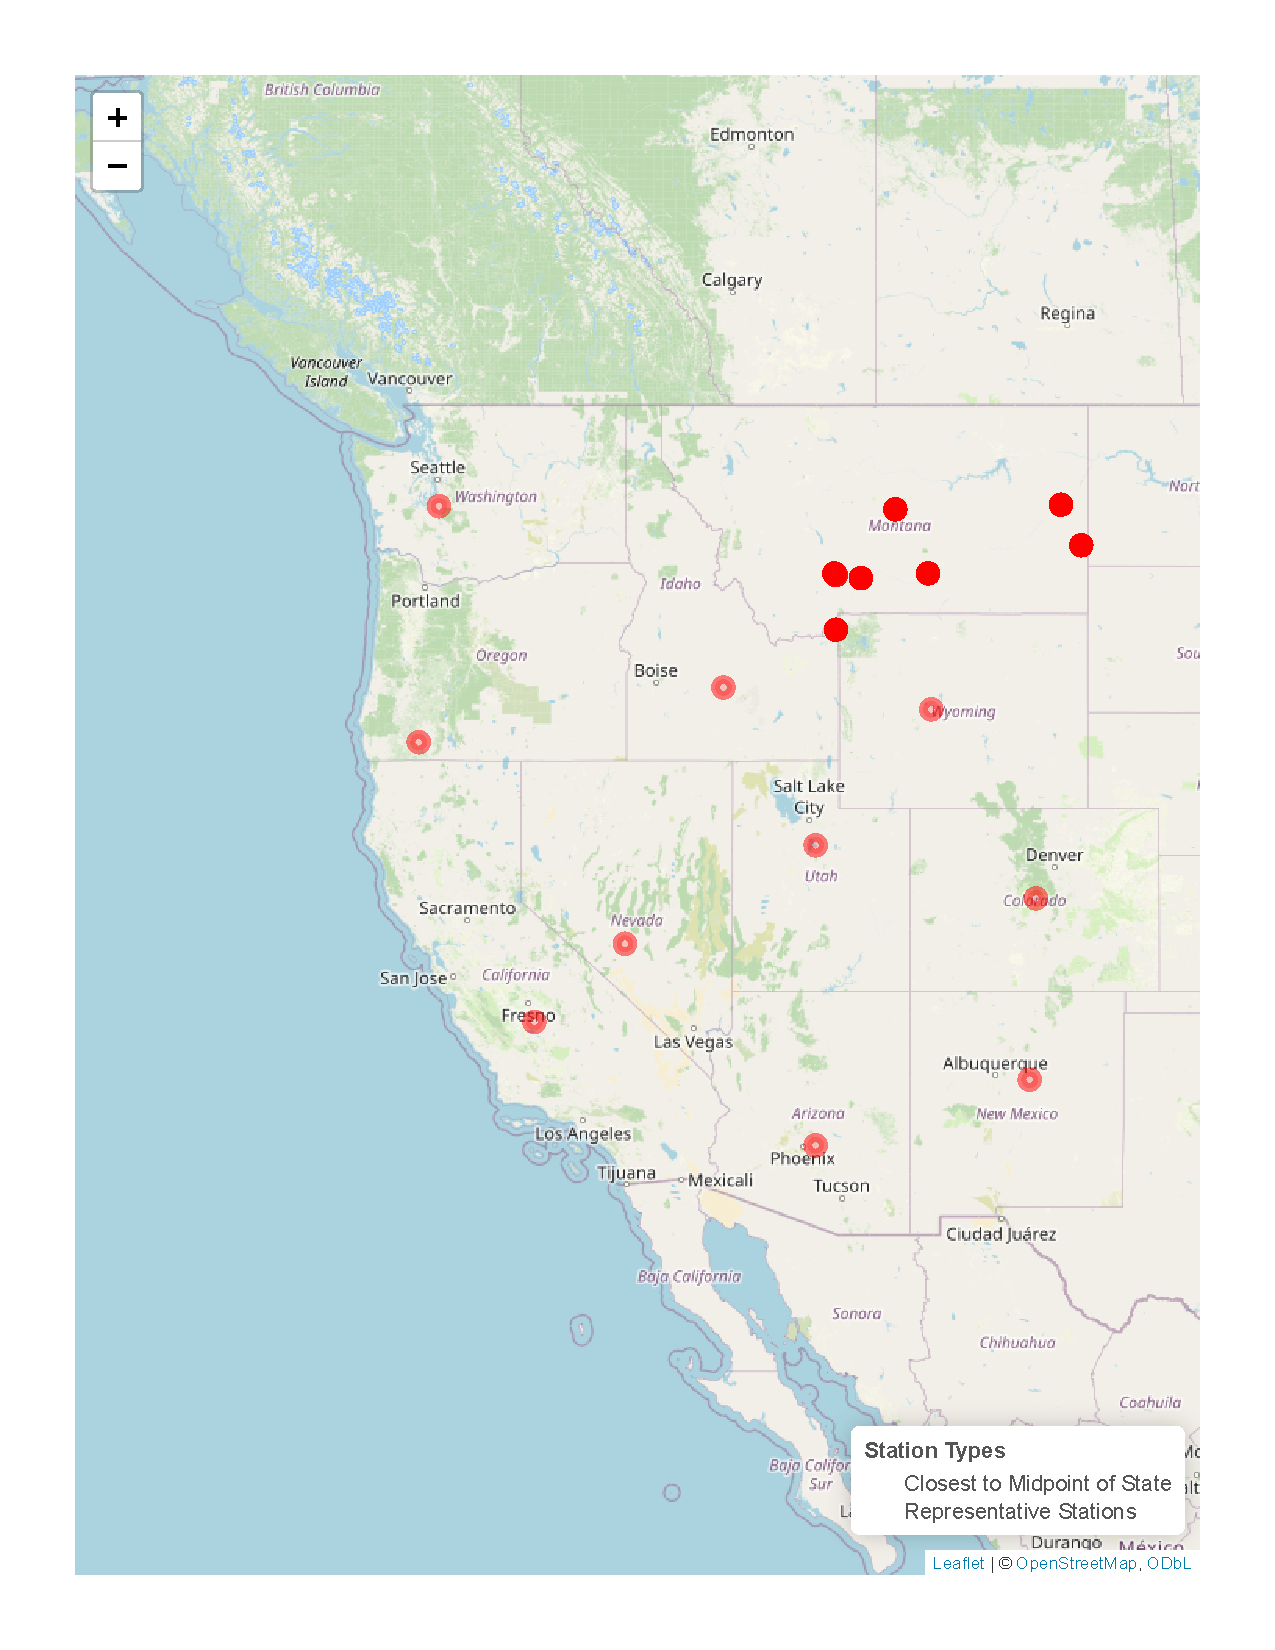
\includegraphics{Lab-5_files/figure-pdf/unnamed-chunk-20-1.pdf}

\subsection{Question 4: Means of means}\label{question-4-means-of-means}

\begin{Shaded}
\begin{Highlighting}[]
\NormalTok{state\_summary }\OtherTok{\textless{}{-}}\NormalTok{ met }\SpecialCharTok{|\textgreater{}}
  \FunctionTok{group\_by}\NormalTok{(STATE) }\SpecialCharTok{|\textgreater{}}
  \FunctionTok{summarise}\NormalTok{(}
    \AttributeTok{avg\_temp =} \FunctionTok{mean}\NormalTok{(temp, }\AttributeTok{na.rm =} \ConstantTok{TRUE}\NormalTok{),}
    \AttributeTok{avg\_wind.sp =} \FunctionTok{mean}\NormalTok{(wind.sp, }\AttributeTok{na.rm =} \ConstantTok{TRUE}\NormalTok{),}
    \AttributeTok{avg\_atm.press =} \FunctionTok{mean}\NormalTok{(atm.press, }\AttributeTok{na.rm =} \ConstantTok{TRUE}\NormalTok{),}
    \AttributeTok{.groups =} \StringTok{\textquotesingle{}drop\textquotesingle{}}
\NormalTok{  )}
\end{Highlighting}
\end{Shaded}

\begin{Shaded}
\begin{Highlighting}[]
\NormalTok{state\_summary }\OtherTok{\textless{}{-}}\NormalTok{ state\_summary }\SpecialCharTok{|\textgreater{}}
  \FunctionTok{mutate}\NormalTok{(}
    \AttributeTok{temp\_level =} \FunctionTok{case\_when}\NormalTok{(}
\NormalTok{      avg\_temp }\SpecialCharTok{\textless{}} \DecValTok{20} \SpecialCharTok{\textasciitilde{}} \StringTok{"Low"}\NormalTok{,}
\NormalTok{      avg\_temp }\SpecialCharTok{\textgreater{}=} \DecValTok{20} \SpecialCharTok{\&}\NormalTok{ avg\_temp }\SpecialCharTok{\textless{}} \DecValTok{25} \SpecialCharTok{\textasciitilde{}} \StringTok{"Mid"}\NormalTok{,}
\NormalTok{      avg\_temp }\SpecialCharTok{\textgreater{}=} \DecValTok{25} \SpecialCharTok{\textasciitilde{}} \StringTok{"High"}\NormalTok{,}
      \ConstantTok{TRUE} \SpecialCharTok{\textasciitilde{}} \ConstantTok{NA\_character\_}
\NormalTok{    )}
\NormalTok{  )}
\end{Highlighting}
\end{Shaded}

\begin{Shaded}
\begin{Highlighting}[]
\CommentTok{\#generating rest of summary table}
\NormalTok{summary\_table }\OtherTok{\textless{}{-}}\NormalTok{ state\_summary }\SpecialCharTok{|\textgreater{}}
\FunctionTok{group\_by}\NormalTok{(temp\_level) }\SpecialCharTok{|\textgreater{}}
\FunctionTok{summarise}\NormalTok{(}
    \AttributeTok{num\_entries =} \FunctionTok{n}\NormalTok{(),}
    \AttributeTok{num\_na\_entries =} \FunctionTok{sum}\NormalTok{(}\FunctionTok{is.na}\NormalTok{(avg\_temp)),}
    \AttributeTok{num\_stations =} \FunctionTok{n\_distinct}\NormalTok{(STATE),  }\CommentTok{\# Assuming each State corresponds to one station}
    \AttributeTok{num\_states =} \FunctionTok{n}\NormalTok{(),  }\CommentTok{\# Number of unique states in each temperature level}
    \AttributeTok{mean\_temp =} \FunctionTok{mean}\NormalTok{(avg\_temp, }\AttributeTok{na.rm =} \ConstantTok{TRUE}\NormalTok{),}
    \AttributeTok{mean\_wind\_speed =} \FunctionTok{mean}\NormalTok{(avg\_wind.sp, }\AttributeTok{na.rm =} \ConstantTok{TRUE}\NormalTok{),}
    \AttributeTok{mean\_atm\_pressure =} \FunctionTok{mean}\NormalTok{(avg\_atm.press, }\AttributeTok{na.rm =} \ConstantTok{TRUE}\NormalTok{),}
    \AttributeTok{.groups =} \StringTok{\textquotesingle{}drop\textquotesingle{}}
\NormalTok{  )}
\FunctionTok{print}\NormalTok{(summary\_table)}
\end{Highlighting}
\end{Shaded}

\begin{verbatim}
# A tibble: 3 x 8
  temp_level num_entries num_na_entries num_stations num_states mean_temp
  <chr>            <int>          <int>        <int>      <int>     <dbl>
1 High                14              0           14         14      27.2
2 Low                  8              0            8          8      19.4
3 Mid                 26              0           26         26      22.7
# i 2 more variables: mean_wind_speed <dbl>, mean_atm_pressure <dbl>
\end{verbatim}




\end{document}
